\documentclass[12pt,a4paper]{article}
\usepackage[colorlinks=true]{hyperref}
\usepackage[utf8]{inputenc}
\usepackage{graphicx}
\usepackage{amsmath}
\usepackage[czech]{babel}
\textwidth 16cm \textheight 24.6cm
\topmargin -1.3cm 
\oddsidemargin 0cm
\pagestyle{empty}
\begin{document}
\title{Měření mikrostruktur nosičů informací -- CD jako difrakční mřížka}
\author{V. Pospíšil\\Fakulta jaderná a fyzikálně inženýrská ČVUT\\gdermog@seznam.cz}
\date{}
\maketitle
\thispagestyle{empty}
\begin{abstract}
Práce představuje použití difrakčního obrazce k změření hustoty záznamu na zvukových nosičích -- CD. Nosič má podobnou strukturu jako klasické vinylové gramofonové desky a \uv{drážky} fungují obdobně jako difrakční mřížka. Cílem je stanovit mřížkovou konstantu zvukového nosiče. K vytvoření obrazce je použit He-Ne laser.
\end{abstract}

\section{Úvod}
Difrakční mřížka -- soustava $N$ identických ekvidistantních štěrbin (vrypů). Může
světlo buď propouštět, nebo odrážet. Tento pokus je zaměřen pouze na difrakční
mřížku, která světlo odráží. Dopadá-li na reflexní mřížku paprsek, pak každý
bod mřížky je podle Huygensova principu zdrojem kulových vlnoploch, tedy
zdrojem rozbíhavých paprsků (viz obr. \ref{fig1}). Jejich interferencí 
vznikají charakteristická maxima a minima. 

\begin{figure}[ht]
\centering
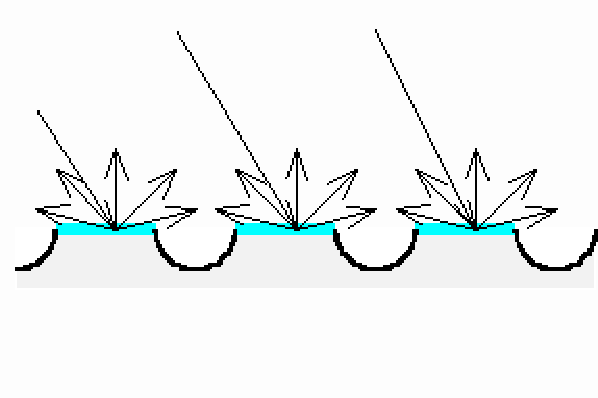
\includegraphics[width=0.48\textwidth]{Image2}
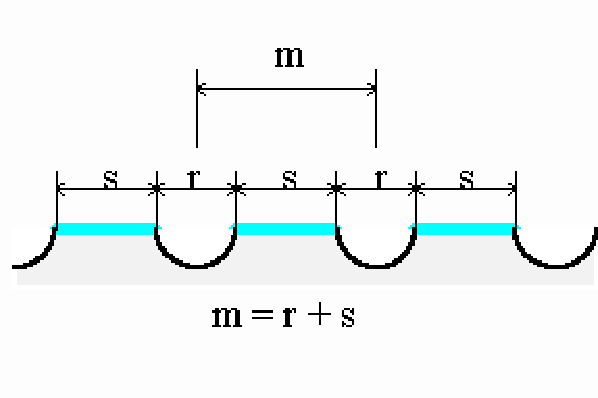
\includegraphics[width=0.48\textwidth]{Image1}
\vspace{-24pt}
\caption{CD jako difrakční mřížka} \label{fig1}
\end{figure} 


\section{Difrakční mřížka}
Difrakční mřížka (\uv{reflexní}) je deska z určitého materiálu, do níž jsou velmi
přesně vyryty identické ekvidistantní vrypy. Předpokládejme, že všechny vrypy
mají stejnou šířku~$r$ a~jsou od sebe stejně vzdáleny. Mezeru mezi dvěma vrypy
nazveme proužek (místo ne\-po\-ru\-še\-né\-ho povrchu desky) a~jeho šířku označíme~$s$.
Soustavu vryp + proužek nazveme difrakční element. Vzdálenost stejně položených
částí dvou sousedních difrakčních elementů je $m=r+s$, kde $m$ je mřížková
konstanta (perioda mřížky). Pro vytvoření si názornější představy o hodnotě mřížkové
konstanty se často používá její převrácené hodnoty 1/m. Ta vyjadřuje počet
difrakčních elementů mřížky na jednotku délky. $N$ vyjadřuje celkový počet
difrakčních elementů mřížky.

Dopadá-li paprsek na mřížku kolmo, platí pro jednotlivá maxima rovnice 
\begin{equation}
m\sin\alpha =n\cdot \lambda \, ,
\end{equation}
teoreticky je tedy možné získat mřížkovou konstantu změřením jediného úhlu. Je ovšem třeba počítat s nepřesnostmi. 
Které hodnoty byly odečítány, je patrné z obrázku \ref{fig2}:

\begin{figure}[ht]
\centering
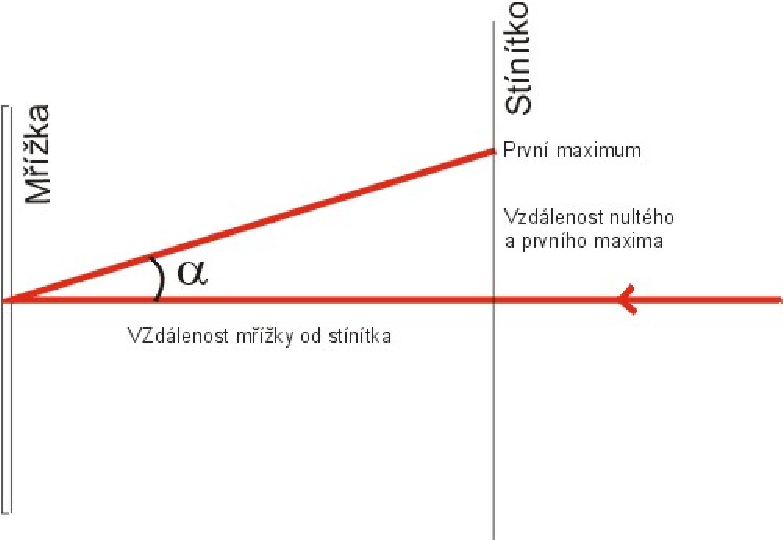
\includegraphics[width=0.8\textwidth]{Image3}
\caption{Difrakční jev}
\end{figure} \label{fig2}


\section{Experimentální uspořádání}
Pro měření (viz obr. \ref{fig3}) byl použit standardní červený He-Ne laser s~vlnovou délkou  $\rm 632,\!8\,nm$, CD a stínítko, jež tvořil list tuhého papíru,
bylo upevněno pomocí jednoduchých stojanů. Odečítání vzdáleností se provádělo
pomocí kružítka s dvěma hroty a~kovového pásma (viz obrázek). Takto \uv{na koleně} sestavená aparatura samozřejmě nemůže zajistit dostatečnou
přesnost, nicméně s~ní lze dosáhnout alespoň řádově správných vý\-sle\-dků. Na
obrázku jsou zaznamenány hlavní vnesené nepřesnosti.

Provedena byla  čtyři měření -- pro dvě různé
vzdálenosti stínítka od mřížky byly změřeny vzdálenosti maxima nultého od
maxima prvního a druhého řádu a spočítány úhly, které spolu paprsky svírají.
Pomocí výše zmíněné rovnice pak byla určena experimentálně naměřená hodnota mřížkové konstanty
pro každé měření.

\begin{figure}[h]
\centering
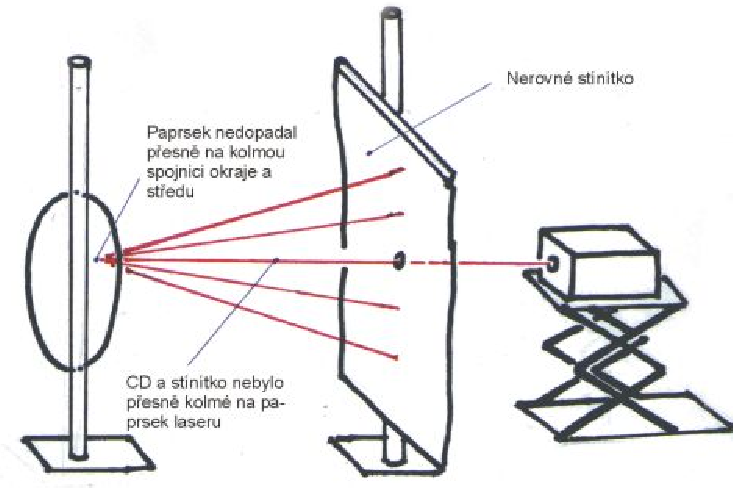
\includegraphics[width=0.72\textwidth]{Image4}
\caption{Experimentální sestava}
\end{figure} \label{fig3}


\section{Výsledky a diskuze}
V tabulce č.~\ref{tab:namerene} jsou zaznamenány naměřené vzdálenosti maxim vzhledem 
ke vzdálenosti CD od stínítka. V posledním sloupci vidíme
vlastní hodnoty mřížkové konstanty v nanometrech.

\begin{table}
\begin{center}
\caption{\label{tab:namerene}Tabulka naměřených hodnot a určených odpovídajících mřížkových konstant}~\\
\begin{tabular}{|c|r|r|r|}\hline
\rule[-3ex]{0pt}{7.5ex}	 {\sf $\rm Maximum\:\check{c}.$}
	&{\sf $\dfrac{\rm Poloha\:maxima}{\rm mm}$}
	&{\sf $\dfrac{\rm Vzd\acute{a}lenost\:st\acute{ı}n\acute{ı}tka}{\rm mm}$}
	&{\sf $\dfrac{\rm M\check{r}\acute{ı}\check{z}kov\acute{a}\:konstanta}{\rm nm}$}
\\\hline
	 {\sf $1$}
	&{\sf $20,\!5$}
	&{\sf $50$}
	&{\sf $1\,668$}
\\\hline
	 {\sf $2$}
	&{\sf $65,\!5$}
	&{\sf $50$}
	&{\sf $1\,597$}
\\\hline
	 {\sf $1$}
	&{\sf $29,\!0$}
	&{\sf $65$}
	&{\sf $1\,553$}
\\\hline
	 {\sf $2$}
	&{\sf $83,\!5$}
	&{\sf $65$}
	&{\sf $1\,604$}
\\\hline
\end{tabular}
\end{center}
\end{table}

Statisticky určená hodnota mřížkové konstanty je $\left(1\,605\pm 48\right){\rm nm}$. Pokud se pak po\-dí\-vá\-me na chyby určení jednotlivých veličin, pak se nám chyba zvýší o~systematickou a~výsledná hodnota je po zaokrouhlení $\left(1,\!6\pm 0,1\right){\rm \mu{}m}$. Hodnotu bychom mohli dále zpře\-s\-nit opakovanými měřeními pro různé vzdálenosti stínítek, určování více maxim, pokud jsou viditelná, a využití různých vlnových délek laserů. Další možností by bylo určovat mřížkovou konstantu na různých místech CD pro ověření, jestli je mřížková konstanta skutečně konstantní v rámci celého povrchu. V dalších měřeních v budoucnu bychom se mohli zaměřit na další podobná paměťová média jako DVD a porovnat hustotu jejich vrypů s~CD.


\section{Závěr}
Experimentálně určená hodnota mřížkové konstanty na povrchu CD je $\left(1,\!6\pm 0,\!1\right){\rm \mu{}m}$. Tato hodnota v rámci chyb měření odpovídá výrobcem udávané, která je $\rm 1\,600\,nm$.


\section*{Poděkování}
Děkuji jménem všech účastníků Vojtěchu Svobodovi za to, že pořádá Týden vědy na Jaderce (dříve Fyzikální týden), díky kterému jsme se mohli seznámit s tímto tématem. Pokud jste dočetli až takto daleko, tak současně gratulujeme pozorné čtenářce či čtenáři. Původní text byl redakčně změněn, abyste měli ještě o něco lepší příklad pro své zpracování. A skutečně nepřesahujte 4 strany, když píšete svůj článek do sborníku.

\begin{thebibliography}{99}
\bibitem{cd1}T. Nedvěd. {\it Pozorujeme spektra}. \href{http://www.ped.muni.cz/wphy/NEDVED/cd1.htm}{http://www.ped.muni.cz/wphy/NEDVED/cd1.htm}
\bibitem{kuhn}Kelin J. Kuhn. {\it Audio Compact Disk -- An Introduction.} \href{http://www.ee.washington.edu/conselec/CE/kuhn/cdaudio/95x6.htm}{http://www.ee.washington.edu/conselec/CE/kuhn/cdaudio/95x6.htm}.
\end{thebibliography}

\end{document}
